In questa sezione sono riportati i risultati del confronto tra le normali climatiche di stazione elaborate come illustrato nel paragrafo precedente e quelle ricostruite con approccio \emph{leave one out} e interpolazione geografica LWLR in funzione di quota, distanza dal mare, orientamento e pendenza del terreno secondo il metodo usato nel lavoro del 2014. I dati geografici di distanza dal mare, pendenza e orientamento sono stati calcolati con il DEM GTOPO30~\cite{geschNewLandSurface1999}, che ha risoluzione di \qty{30}{\arcsecond}: si è scelto per il momento lo stesso livello di dettaglio del lavoro precedente per evitare di incorrere nei problemi che una risoluzione troppo elevata potrebbe portare. L'obiettivo è ottenere una stima preliminare sulla fattibilità della produzione di un dataset grigliato delle normali interpolate e sondare i fattori che influenzano le prestazioni del modello in questa fase iniziale. In quanto segue, con il termine ``BIAS'' o ``scostamento'' si indica la differenza tra le climatologie da modello e da osservazioni, mentre con ``MAE'' ed ``RMSE'' rispettivamente la media del valore assoluto del BIAS e la radice della media dei BIAS quadrati.

\begin{table}[ht]
  \centering
  \begin{adjustbox}{max width=\textwidth}
    \begin{threeparttable}
      \caption{Accuratezza delle climatologie stimate per le temperature minime e massime delle stazioni del centro-nord Italia a confronto con i risultati precedenti.}\label{tab:diffs-mese-ita}
      
\begin{tabular}[t]{rrrrrrr}
\toprule
\multicolumn{1}{c}{ } & \multicolumn{3}{c}{TM7.5 [\unit{\degreeCelsius}]} & \multicolumn{3}{c}{TM14\tnote{*} [\unit{\degreeCelsius}]} \\
\cmidrule(l{3pt}r{3pt}){2-4} \cmidrule(l{3pt}r{3pt}){5-7}
Mese & BIAS & MAE & RMSE & BIAS & MAE & RMSE\\
\midrule
1 & -0.05 & 0.64 & 0.87 & -0.04 & 0.77 & 1.01\\
2 & -0.05 & 0.58 & 0.77 & -0.04 & 0.69 & 0.90\\
3 & -0.05 & 0.54 & 0.73 & -0.03 & 0.60 & 0.78\\
4 & -0.03 & 0.52 & 0.71 & -0.03 & 0.58 & 0.74\\
5 & -0.02 & 0.51 & 0.69 & -0.02 & 0.58 & 0.74\\
\addlinespace
6 & -0.03 & 0.55 & 0.74 & -0.01 & 0.62 & 0.79\\
7 & -0.04 & 0.58 & 0.78 & -0.02 & 0.66 & 0.85\\
8 & -0.03 & 0.58 & 0.77 & -0.02 & 0.65 & 0.84\\
9 & -0.02 & 0.54 & 0.73 & -0.02 & 0.62 & 0.79\\
10 & 0.00 & 0.52 & 0.69 & -0.02 & 0.63 & 0.81\\
\addlinespace
11 & -0.02 & 0.55 & 0.73 & -0.03 & 0.67 & 0.86\\
12 & -0.05 & 0.66 & 0.89 & -0.04 & 0.78 & 1.03\\
\bottomrule
\end{tabular}
      \begin{tablenotes}
      \item[*] Tabella 1 da~\cite[p.~10]{brunettiHighresolutionTemperatureClimatology2014}. Le statistiche d'errore riguardano le temperature medie per il trentennio 1961--1990 e l'intera penisola.
      \end{tablenotes}
    \end{threeparttable}
  \end{adjustbox}
\end{table}

\begin{figure}[ht]
  \centering
  % Created by tikzDevice version 0.12.6 on 2025-04-07 16:54:18
% !TEX encoding = UTF-8 Unicode
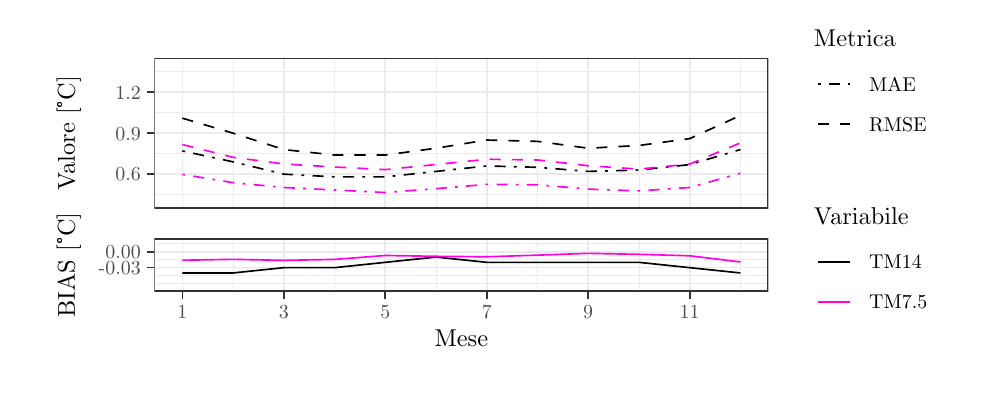
\begin{tikzpicture}[x=1pt,y=1pt]
\definecolor{fillColor}{RGB}{255,255,255}
\path[use as bounding box,fill=fillColor] (0,0) rectangle (341.43,128.04);
\begin{scope}
\path[clip] (  0.00,  0.00) rectangle (341.43,128.04);
\definecolor{drawColor}{RGB}{255,255,255}

\path[draw=drawColor,line width= 0.6pt,line join=round,line cap=round,fill=fillColor] ( -0.00,  0.00) rectangle (341.43,128.04);
\end{scope}
\begin{scope}
\path[clip] (  5.50, 57.28) rectangle (335.93,122.54);
\definecolor{drawColor}{RGB}{255,255,255}
\definecolor{fillColor}{RGB}{255,255,255}

\path[draw=drawColor,line width= 0.6pt,line join=round,line cap=round,fill=fillColor] (  5.50, 57.28) rectangle (335.93,122.54);
\end{scope}
\begin{scope}
\path[clip] (  5.50,  5.50) rectangle (335.93, 57.28);
\definecolor{drawColor}{RGB}{255,255,255}
\definecolor{fillColor}{RGB}{255,255,255}

\path[draw=drawColor,line width= 0.6pt,line join=round,line cap=round,fill=fillColor] (  5.50,  5.50) rectangle (335.93, 57.28);
\end{scope}
\begin{scope}
\path[clip] ( 45.82, 62.78) rectangle (267.62,117.04);
\definecolor{fillColor}{RGB}{255,255,255}

\path[fill=fillColor] ( 45.82, 62.78) rectangle (267.62,117.04);
\definecolor{drawColor}{gray}{0.92}

\path[draw=drawColor,line width= 0.3pt,line join=round] ( 45.82, 67.71) --
	(267.62, 67.71);

\path[draw=drawColor,line width= 0.3pt,line join=round] ( 45.82, 82.51) --
	(267.62, 82.51);

\path[draw=drawColor,line width= 0.3pt,line join=round] ( 45.82, 97.31) --
	(267.62, 97.31);

\path[draw=drawColor,line width= 0.3pt,line join=round] ( 45.82,112.10) --
	(267.62,112.10);

\path[draw=drawColor,line width= 0.3pt,line join=round] ( 74.23, 62.78) --
	( 74.23,117.04);

\path[draw=drawColor,line width= 0.3pt,line join=round] (110.89, 62.78) --
	(110.89,117.04);

\path[draw=drawColor,line width= 0.3pt,line join=round] (147.56, 62.78) --
	(147.56,117.04);

\path[draw=drawColor,line width= 0.3pt,line join=round] (184.22, 62.78) --
	(184.22,117.04);

\path[draw=drawColor,line width= 0.3pt,line join=round] (220.88, 62.78) --
	(220.88,117.04);

\path[draw=drawColor,line width= 0.3pt,line join=round] (257.54, 62.78) --
	(257.54,117.04);

\path[draw=drawColor,line width= 0.6pt,line join=round] ( 45.82, 75.11) --
	(267.62, 75.11);

\path[draw=drawColor,line width= 0.6pt,line join=round] ( 45.82, 89.91) --
	(267.62, 89.91);

\path[draw=drawColor,line width= 0.6pt,line join=round] ( 45.82,104.71) --
	(267.62,104.71);

\path[draw=drawColor,line width= 0.6pt,line join=round] ( 55.90, 62.78) --
	( 55.90,117.04);

\path[draw=drawColor,line width= 0.6pt,line join=round] ( 92.56, 62.78) --
	( 92.56,117.04);

\path[draw=drawColor,line width= 0.6pt,line join=round] (129.22, 62.78) --
	(129.22,117.04);

\path[draw=drawColor,line width= 0.6pt,line join=round] (165.89, 62.78) --
	(165.89,117.04);

\path[draw=drawColor,line width= 0.6pt,line join=round] (202.55, 62.78) --
	(202.55,117.04);

\path[draw=drawColor,line width= 0.6pt,line join=round] (239.21, 62.78) --
	(239.21,117.04);
\definecolor{drawColor}{RGB}{0,0,0}

\path[draw=drawColor,line width= 0.6pt,dash pattern=on 1pt off 3pt on 4pt off 3pt ,line join=round] ( 55.90, 83.50) --
	( 74.23, 79.55) --
	( 92.56, 75.11) --
	(110.89, 74.12) --
	(129.22, 74.12) --
	(147.56, 76.10) --
	(165.89, 78.07) --
	(184.22, 77.58) --
	(202.55, 76.10) --
	(220.88, 76.59) --
	(239.21, 78.56) --
	(257.54, 83.99);

\path[draw=drawColor,line width= 0.6pt,dash pattern=on 4pt off 4pt ,line join=round] ( 55.90, 95.33) --
	( 74.23, 89.91) --
	( 92.56, 83.99) --
	(110.89, 82.02) --
	(129.22, 82.02) --
	(147.56, 84.48) --
	(165.89, 87.44) --
	(184.22, 86.95) --
	(202.55, 84.48) --
	(220.88, 85.47) --
	(239.21, 87.94) --
	(257.54, 96.32);
\definecolor{drawColor}{RGB}{255,0,230}

\path[draw=drawColor,line width= 0.6pt,dash pattern=on 1pt off 3pt on 4pt off 3pt ,line join=round] ( 55.90, 75.01) --
	( 74.23, 72.04) --
	( 92.56, 70.28) --
	(110.89, 69.39) --
	(129.22, 68.46) --
	(147.56, 69.87) --
	(165.89, 71.42) --
	(184.22, 71.27) --
	(202.55, 69.71) --
	(220.88, 69.06) --
	(239.21, 70.29) --
	(257.54, 75.43);

\path[draw=drawColor,line width= 0.6pt,dash pattern=on 4pt off 4pt ,line join=round] ( 55.90, 85.81) --
	( 74.23, 81.19) --
	( 92.56, 78.78) --
	(110.89, 77.69) --
	(129.22, 76.75) --
	(147.56, 78.60) --
	(165.89, 80.49) --
	(184.22, 80.24) --
	(202.55, 78.15) --
	(220.88, 76.93) --
	(239.21, 78.75) --
	(257.54, 86.39);
\definecolor{drawColor}{gray}{0.20}

\path[draw=drawColor,line width= 0.6pt,line join=round,line cap=round] ( 45.82, 62.78) rectangle (267.62,117.04);
\end{scope}
\begin{scope}
\path[clip] (  0.00,  0.00) rectangle (341.43,128.04);
\definecolor{drawColor}{gray}{0.30}

\node[text=drawColor,anchor=base east,inner sep=0pt, outer sep=0pt, scale=  0.72] at ( 40.87, 72.65) {0.6};

\node[text=drawColor,anchor=base east,inner sep=0pt, outer sep=0pt, scale=  0.72] at ( 40.87, 87.45) {0.9};

\node[text=drawColor,anchor=base east,inner sep=0pt, outer sep=0pt, scale=  0.72] at ( 40.87,102.24) {1.2};
\end{scope}
\begin{scope}
\path[clip] (  0.00,  0.00) rectangle (341.43,128.04);
\definecolor{drawColor}{gray}{0.20}

\path[draw=drawColor,line width= 0.6pt,line join=round] ( 43.07, 75.11) --
	( 45.82, 75.11);

\path[draw=drawColor,line width= 0.6pt,line join=round] ( 43.07, 89.91) --
	( 45.82, 89.91);

\path[draw=drawColor,line width= 0.6pt,line join=round] ( 43.07,104.71) --
	( 45.82,104.71);
\end{scope}
\begin{scope}
\path[clip] (  0.00,  0.00) rectangle (341.43,128.04);
\definecolor{drawColor}{RGB}{0,0,0}

\node[text=drawColor,rotate= 90.00,anchor=base,inner sep=0pt, outer sep=0pt, scale=  0.88] at ( 17.06, 89.91) {Valore [\textdegree C]};
\end{scope}
\begin{scope}
\path[clip] ( 45.82, 32.79) rectangle (267.62, 51.78);
\definecolor{fillColor}{RGB}{255,255,255}

\path[fill=fillColor] ( 45.82, 32.79) rectangle (267.62, 51.78);
\definecolor{drawColor}{gray}{0.92}

\path[draw=drawColor,line width= 0.3pt,line join=round] ( 45.82, 35.57) --
	(267.62, 35.57);

\path[draw=drawColor,line width= 0.3pt,line join=round] ( 45.82, 38.45) --
	(267.62, 38.45);

\path[draw=drawColor,line width= 0.3pt,line join=round] ( 45.82, 44.20) --
	(267.62, 44.20);

\path[draw=drawColor,line width= 0.3pt,line join=round] ( 45.82, 49.96) --
	(267.62, 49.96);

\path[draw=drawColor,line width= 0.3pt,line join=round] ( 74.23, 32.79) --
	( 74.23, 51.78);

\path[draw=drawColor,line width= 0.3pt,line join=round] (110.89, 32.79) --
	(110.89, 51.78);

\path[draw=drawColor,line width= 0.3pt,line join=round] (147.56, 32.79) --
	(147.56, 51.78);

\path[draw=drawColor,line width= 0.3pt,line join=round] (184.22, 32.79) --
	(184.22, 51.78);

\path[draw=drawColor,line width= 0.3pt,line join=round] (220.88, 32.79) --
	(220.88, 51.78);

\path[draw=drawColor,line width= 0.3pt,line join=round] (257.54, 32.79) --
	(257.54, 51.78);

\path[draw=drawColor,line width= 0.6pt,line join=round] ( 45.82, 41.32) --
	(267.62, 41.32);

\path[draw=drawColor,line width= 0.6pt,line join=round] ( 45.82, 47.08) --
	(267.62, 47.08);

\path[draw=drawColor,line width= 0.6pt,line join=round] ( 55.90, 32.79) --
	( 55.90, 51.78);

\path[draw=drawColor,line width= 0.6pt,line join=round] ( 92.56, 32.79) --
	( 92.56, 51.78);

\path[draw=drawColor,line width= 0.6pt,line join=round] (129.22, 32.79) --
	(129.22, 51.78);

\path[draw=drawColor,line width= 0.6pt,line join=round] (165.89, 32.79) --
	(165.89, 51.78);

\path[draw=drawColor,line width= 0.6pt,line join=round] (202.55, 32.79) --
	(202.55, 51.78);

\path[draw=drawColor,line width= 0.6pt,line join=round] (239.21, 32.79) --
	(239.21, 51.78);
\definecolor{drawColor}{RGB}{0,0,0}

\path[draw=drawColor,line width= 0.6pt,line join=round] ( 55.90, 39.41) --
	( 74.23, 39.41) --
	( 92.56, 41.32) --
	(110.89, 41.32) --
	(129.22, 43.24) --
	(147.56, 45.16) --
	(165.89, 43.24) --
	(184.22, 43.24) --
	(202.55, 43.24) --
	(220.88, 43.24) --
	(239.21, 41.32) --
	(257.54, 39.41);
\definecolor{drawColor}{RGB}{255,0,230}

\path[draw=drawColor,line width= 0.6pt,line join=round] ( 55.90, 44.01) --
	( 74.23, 44.33) --
	( 92.56, 43.96) --
	(110.89, 44.30) --
	(129.22, 45.72) --
	(147.56, 45.42) --
	(165.89, 45.25) --
	(184.22, 45.84) --
	(202.55, 46.49) --
	(220.88, 46.14) --
	(239.21, 45.61) --
	(257.54, 43.38);
\definecolor{drawColor}{gray}{0.20}

\path[draw=drawColor,line width= 0.6pt,line join=round,line cap=round] ( 45.82, 32.79) rectangle (267.62, 51.78);
\end{scope}
\begin{scope}
\path[clip] (  0.00,  0.00) rectangle (341.43,128.04);
\definecolor{drawColor}{gray}{0.30}

\node[text=drawColor,anchor=base east,inner sep=0pt, outer sep=0pt, scale=  0.72] at ( 40.87, 38.86) {-0.03};

\node[text=drawColor,anchor=base east,inner sep=0pt, outer sep=0pt, scale=  0.72] at ( 40.87, 44.62) {0.00};
\end{scope}
\begin{scope}
\path[clip] (  0.00,  0.00) rectangle (341.43,128.04);
\definecolor{drawColor}{gray}{0.20}

\path[draw=drawColor,line width= 0.6pt,line join=round] ( 43.07, 41.32) --
	( 45.82, 41.32);

\path[draw=drawColor,line width= 0.6pt,line join=round] ( 43.07, 47.08) --
	( 45.82, 47.08);
\end{scope}
\begin{scope}
\path[clip] (  0.00,  0.00) rectangle (341.43,128.04);
\definecolor{drawColor}{gray}{0.20}

\path[draw=drawColor,line width= 0.6pt,line join=round] ( 55.90, 30.04) --
	( 55.90, 32.79);

\path[draw=drawColor,line width= 0.6pt,line join=round] ( 92.56, 30.04) --
	( 92.56, 32.79);

\path[draw=drawColor,line width= 0.6pt,line join=round] (129.22, 30.04) --
	(129.22, 32.79);

\path[draw=drawColor,line width= 0.6pt,line join=round] (165.89, 30.04) --
	(165.89, 32.79);

\path[draw=drawColor,line width= 0.6pt,line join=round] (202.55, 30.04) --
	(202.55, 32.79);

\path[draw=drawColor,line width= 0.6pt,line join=round] (239.21, 30.04) --
	(239.21, 32.79);
\end{scope}
\begin{scope}
\path[clip] (  0.00,  0.00) rectangle (341.43,128.04);
\definecolor{drawColor}{gray}{0.30}

\node[text=drawColor,anchor=base,inner sep=0pt, outer sep=0pt, scale=  0.72] at ( 55.90, 22.91) {1};

\node[text=drawColor,anchor=base,inner sep=0pt, outer sep=0pt, scale=  0.72] at ( 92.56, 22.91) {3};

\node[text=drawColor,anchor=base,inner sep=0pt, outer sep=0pt, scale=  0.72] at (129.22, 22.91) {5};

\node[text=drawColor,anchor=base,inner sep=0pt, outer sep=0pt, scale=  0.72] at (165.89, 22.91) {7};

\node[text=drawColor,anchor=base,inner sep=0pt, outer sep=0pt, scale=  0.72] at (202.55, 22.91) {9};

\node[text=drawColor,anchor=base,inner sep=0pt, outer sep=0pt, scale=  0.72] at (239.21, 22.91) {11};
\end{scope}
\begin{scope}
\path[clip] (  0.00,  0.00) rectangle (341.43,128.04);
\definecolor{drawColor}{RGB}{0,0,0}

\node[text=drawColor,anchor=base,inner sep=0pt, outer sep=0pt, scale=  0.88] at (156.72, 12.71) {Mese};
\end{scope}
\begin{scope}
\path[clip] (  0.00,  0.00) rectangle (341.43,128.04);
\definecolor{drawColor}{RGB}{0,0,0}

\node[text=drawColor,rotate= 90.00,anchor=base,inner sep=0pt, outer sep=0pt, scale=  0.88] at ( 17.06, 42.28) {BIAS [\textdegree C]};
\end{scope}
\begin{scope}
\path[clip] (  0.00,  0.00) rectangle (341.43,128.04);
\definecolor{fillColor}{RGB}{255,255,255}

\path[fill=fillColor] (278.62, 80.41) rectangle (330.23,133.59);
\end{scope}
\begin{scope}
\path[clip] (  0.00,  0.00) rectangle (341.43,128.04);
\definecolor{drawColor}{RGB}{0,0,0}

\node[text=drawColor,anchor=base west,inner sep=0pt, outer sep=0pt, scale=  0.88] at (284.12,121.18) {Metrica};
\end{scope}
\begin{scope}
\path[clip] (  0.00,  0.00) rectangle (341.43,128.04);
\definecolor{fillColor}{RGB}{255,255,255}

\path[fill=fillColor] (284.12,100.37) rectangle (298.58,114.82);
\end{scope}
\begin{scope}
\path[clip] (  0.00,  0.00) rectangle (341.43,128.04);
\definecolor{drawColor}{RGB}{0,0,0}

\path[draw=drawColor,line width= 0.6pt,dash pattern=on 1pt off 3pt on 4pt off 3pt ,line join=round] (285.57,107.59) -- (297.13,107.59);
\end{scope}
\begin{scope}
\path[clip] (  0.00,  0.00) rectangle (341.43,128.04);
\definecolor{fillColor}{RGB}{255,255,255}

\path[fill=fillColor] (284.12, 85.91) rectangle (298.58,100.37);
\end{scope}
\begin{scope}
\path[clip] (  0.00,  0.00) rectangle (341.43,128.04);
\definecolor{drawColor}{RGB}{0,0,0}

\path[draw=drawColor,line width= 0.6pt,dash pattern=on 4pt off 4pt ,line join=round] (285.57, 93.14) -- (297.13, 93.14);
\end{scope}
\begin{scope}
\path[clip] (  0.00,  0.00) rectangle (341.43,128.04);
\definecolor{drawColor}{RGB}{0,0,0}

\node[text=drawColor,anchor=base west,inner sep=0pt, outer sep=0pt, scale=  0.72] at (304.08,105.13) {MAE};
\end{scope}
\begin{scope}
\path[clip] (  0.00,  0.00) rectangle (341.43,128.04);
\definecolor{drawColor}{RGB}{0,0,0}

\node[text=drawColor,anchor=base west,inner sep=0pt, outer sep=0pt, scale=  0.72] at (304.08, 90.68) {RMSE};
\end{scope}
\begin{scope}
\path[clip] (  0.00,  0.00) rectangle (341.43,128.04);
\definecolor{fillColor}{RGB}{255,255,255}

\path[fill=fillColor] (278.62, 16.23) rectangle (330.43, 69.41);
\end{scope}
\begin{scope}
\path[clip] (  0.00,  0.00) rectangle (341.43,128.04);
\definecolor{drawColor}{RGB}{0,0,0}

\node[text=drawColor,anchor=base west,inner sep=0pt, outer sep=0pt, scale=  0.88] at (284.12, 57.00) {Variabile};
\end{scope}
\begin{scope}
\path[clip] (  0.00,  0.00) rectangle (341.43,128.04);
\definecolor{fillColor}{RGB}{255,255,255}

\path[fill=fillColor] (284.12, 36.19) rectangle (298.58, 50.64);
\end{scope}
\begin{scope}
\path[clip] (  0.00,  0.00) rectangle (341.43,128.04);
\definecolor{drawColor}{RGB}{0,0,0}

\path[draw=drawColor,line width= 0.6pt,line join=round] (285.57, 43.41) -- (297.13, 43.41);
\end{scope}
\begin{scope}
\path[clip] (  0.00,  0.00) rectangle (341.43,128.04);
\definecolor{fillColor}{RGB}{255,255,255}

\path[fill=fillColor] (284.12, 21.73) rectangle (298.58, 36.19);
\end{scope}
\begin{scope}
\path[clip] (  0.00,  0.00) rectangle (341.43,128.04);
\definecolor{drawColor}{RGB}{255,0,230}

\path[draw=drawColor,line width= 0.6pt,line join=round] (285.57, 28.96) -- (297.13, 28.96);
\end{scope}
\begin{scope}
\path[clip] (  0.00,  0.00) rectangle (341.43,128.04);
\definecolor{drawColor}{RGB}{0,0,0}

\node[text=drawColor,anchor=base west,inner sep=0pt, outer sep=0pt, scale=  0.72] at (304.08, 40.95) {TM14};
\end{scope}
\begin{scope}
\path[clip] (  0.00,  0.00) rectangle (341.43,128.04);
\definecolor{drawColor}{RGB}{0,0,0}

\node[text=drawColor,anchor=base west,inner sep=0pt, outer sep=0pt, scale=  0.72] at (304.08, 26.50) {TM7.5};
\end{scope}
\end{tikzpicture}

  \caption{Confronto tra le statistiche del 2014 e le serie italiane ed estere del dataset prodotto.}\label{fig:diffs-mese-ita}
\end{figure}
La tabella~\ref{tab:diffs-mese-ita} e la figura~\ref{fig:diffs-mese-ita} mostrano le statistiche degli scostamenti del modello per le stazioni del centro-nord Italia, che indicano un consistente scarto tra la capacità del modello di ricostruire le serie di temperature minime rispetto alle massime, in particolare nei mesi estivi e invernali. Ciononostante il bias rimane sempre entro il margine accettabile di \(\pm\qty{0.05}{\degreeCelsius}\). Gli scostamenti assoluti e quadratici delle minime invece sono considerevolmente più alti, a suggerire che rispetto al precedente dataset c'è una maggiore presenza di outliers che non vengono ricostruiti in maniera efficace.

\begin{table}[ht]
  \centering
  \begin{adjustbox}{max width=\textwidth}
    \begin{threeparttable}
      \caption{Accuratezza delle climatologie stimate per le temperature minime e massime delle stazioni francesi, svizzere, austriache e slovene.}\label{tab:bias-non-ita}
      
\begin{tabular}[t]{rrrrrrrrrr}
\toprule
\multicolumn{1}{c}{ } & \multicolumn{3}{c}{TN} & \multicolumn{3}{c}{TX} & \multicolumn{3}{c}{2014\tnote{*}} \\
\cmidrule(l{3pt}r{3pt}){2-4} \cmidrule(l{3pt}r{3pt}){5-7} \cmidrule(l{3pt}r{3pt}){8-10}
Mese & BIAS & MAE & RMSE & BIAS & MAE & RMSE & BIAS & MAE & RMSE\\
\midrule
1 & 0.07 & 0.88 & 1.21 & 0.03 & 0.52 & 0.71 & -0.04 & 0.77 & 1.01\\
2 & 0.07 & 0.84 & 1.14 & 0.04 & 0.49 & 0.64 & -0.04 & 0.69 & 0.90\\
3 & 0.05 & 0.77 & 1.02 & 0.03 & 0.52 & 0.68 & -0.03 & 0.60 & 0.78\\
4 & 0.04 & 0.74 & 0.97 & 0.00 & 0.54 & 0.70 & -0.03 & 0.58 & 0.74\\
5 & 0.05 & 0.67 & 0.87 & 0.00 & 0.55 & 0.72 & -0.02 & 0.58 & 0.74\\
\addlinespace
6 & 0.06 & 0.69 & 0.93 & 0.01 & 0.56 & 0.74 & -0.01 & 0.62 & 0.79\\
7 & 0.07 & 0.74 & 1.00 & 0.02 & 0.59 & 0.77 & -0.02 & 0.66 & 0.85\\
8 & 0.07 & 0.77 & 1.04 & 0.02 & 0.57 & 0.75 & -0.02 & 0.65 & 0.84\\
9 & 0.06 & 0.75 & 1.00 & 0.00 & 0.52 & 0.69 & -0.02 & 0.62 & 0.79\\
10 & 0.05 & 0.75 & 1.00 & -0.05 & 0.49 & 0.63 & -0.02 & 0.63 & 0.81\\
\addlinespace
11 & 0.06 & 0.72 & 0.97 & -0.02 & 0.46 & 0.61 & -0.03 & 0.67 & 0.86\\
12 & 0.06 & 0.84 & 1.15 & 0.01 & 0.53 & 0.73 & -0.04 & 0.78 & 1.03\\
\bottomrule
\end{tabular}
      \begin{tablenotes}
      \item[*] Tabella 1 da~\cite[p.~10]{brunettiHighresolutionTemperatureClimatology2014}. Le statistiche d'errore riguardano le temperature medie per il trentennio 1961--1990 e l'intera penisola.
      \end{tablenotes}
    \end{threeparttable}
  \end{adjustbox}
\end{table}
La situazione è differente se si considerano le stazioni esterne al territorio italiano: in questo caso i bias delle minime sono marcatamente più importanti, probabilmente a causa della maggiore proporzione di stazioni in alta quota di queste regioni. Gli scostamenti assoluti e quadratici sono invece inferiori, indicando che ci sono meno ricostruzioni molto anomale.

È stata poi controllata la presenza di errori sistematici nella procedura di ricostruzione a livello locale. In particolare, vista la numerosa quantità di sorgenti presenti nel dataset, è stata fatta una statistica sulle serie raggruppandole per regione di appartenenza. Il pannello sinistro della figura~\ref{fig:boxplots-ita} mostra come alcuni territori (in particolare Liguria, Lombardia, Piemonte, Toscana e Valle d'Aosta) contribuiscano in maniera più significativa a bias e varianza complessivi. Essendo territori dall'orografia complessa, si è studiata la dipendenza del bias dalla quota: il pannello destro della stessa figura mostra che per le minime lo scostamento complessivo è correlato alla quota, mentre per le massime ne aumenta la dispersione, fino a divenire più importante rispetto a quella delle minime.

\begin{figure}[ht]
  \centering
  % Created by tikzDevice version 0.12.6 on 2025-04-07 20:16:07
% !TEX encoding = UTF-8 Unicode
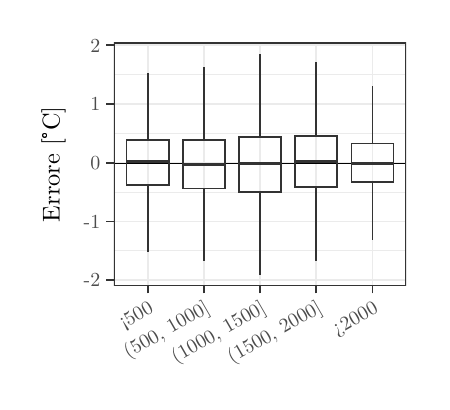
\begin{tikzpicture}[x=1pt,y=1pt]
\definecolor{fillColor}{RGB}{255,255,255}
\path[use as bounding box,fill=fillColor] (0,0) rectangle (142.26,128.04);
\begin{scope}
\path[clip] (  0.00,  0.00) rectangle (142.26,128.04);
\definecolor{drawColor}{RGB}{255,255,255}

\path[draw=drawColor,line width= 0.6pt,line join=round,line cap=round,fill=fillColor] (  0.00,  0.00) rectangle (142.26,128.04);
\end{scope}
\begin{scope}
\path[clip] ( 31.18, 34.79) rectangle (136.76,122.54);
\definecolor{fillColor}{RGB}{255,255,255}

\path[fill=fillColor] ( 31.18, 34.79) rectangle (136.76,122.54);
\definecolor{drawColor}{gray}{0.92}

\path[draw=drawColor,line width= 0.3pt,line join=round] ( 31.18, 47.41) --
	(136.76, 47.41);

\path[draw=drawColor,line width= 0.3pt,line join=round] ( 31.18, 68.63) --
	(136.76, 68.63);

\path[draw=drawColor,line width= 0.3pt,line join=round] ( 31.18, 89.84) --
	(136.76, 89.84);

\path[draw=drawColor,line width= 0.3pt,line join=round] ( 31.18,111.06) --
	(136.76,111.06);

\path[draw=drawColor,line width= 0.6pt,line join=round] ( 31.18, 36.80) --
	(136.76, 36.80);

\path[draw=drawColor,line width= 0.6pt,line join=round] ( 31.18, 58.02) --
	(136.76, 58.02);

\path[draw=drawColor,line width= 0.6pt,line join=round] ( 31.18, 79.24) --
	(136.76, 79.24);

\path[draw=drawColor,line width= 0.6pt,line join=round] ( 31.18,100.45) --
	(136.76,100.45);

\path[draw=drawColor,line width= 0.6pt,line join=round] ( 31.18,121.67) --
	(136.76,121.67);

\path[draw=drawColor,line width= 0.6pt,line join=round] ( 43.36, 34.79) --
	( 43.36,122.54);

\path[draw=drawColor,line width= 0.6pt,line join=round] ( 63.67, 34.79) --
	( 63.67,122.54);

\path[draw=drawColor,line width= 0.6pt,line join=round] ( 83.97, 34.79) --
	( 83.97,122.54);

\path[draw=drawColor,line width= 0.6pt,line join=round] (104.28, 34.79) --
	(104.28,122.54);

\path[draw=drawColor,line width= 0.6pt,line join=round] (124.58, 34.79) --
	(124.58,122.54);
\definecolor{drawColor}{RGB}{0,0,0}

\path[draw=drawColor,line width= 0.1pt,line join=round] ( 31.18, 79.24) -- (136.76, 79.24);
\definecolor{drawColor}{gray}{0.20}

\path[draw=drawColor,line width= 0.6pt,line join=round] ( 43.36, 87.36) -- ( 43.36,111.63);

\path[draw=drawColor,line width= 0.6pt,line join=round] ( 43.36, 71.17) -- ( 43.36, 46.90);

\path[draw=drawColor,line width= 0.6pt] ( 35.75, 87.36) --
	( 35.75, 71.17) --
	( 50.98, 71.17) --
	( 50.98, 87.36) --
	( 35.75, 87.36) --
	cycle;

\path[draw=drawColor,line width= 1.1pt] ( 35.75, 79.57) -- ( 50.98, 79.57);

\path[draw=drawColor,line width= 0.6pt,line join=round] ( 63.67, 87.47) -- ( 63.67,113.78);

\path[draw=drawColor,line width= 0.6pt,line join=round] ( 63.67, 69.89) -- ( 63.67, 43.61);

\path[draw=drawColor,line width= 0.6pt] ( 56.05, 87.47) --
	( 56.05, 69.89) --
	( 71.28, 69.89) --
	( 71.28, 87.47) --
	( 56.05, 87.47) --
	cycle;

\path[draw=drawColor,line width= 1.1pt] ( 56.05, 78.47) -- ( 71.28, 78.47);

\path[draw=drawColor,line width= 0.6pt,line join=round] ( 83.97, 88.64) -- ( 83.97,118.55);

\path[draw=drawColor,line width= 0.6pt,line join=round] ( 83.97, 68.69) -- ( 83.97, 38.78);

\path[draw=drawColor,line width= 0.6pt] ( 76.36, 88.64) --
	( 76.36, 68.69) --
	( 91.59, 68.69) --
	( 91.59, 88.64) --
	( 76.36, 88.64) --
	cycle;

\path[draw=drawColor,line width= 1.1pt] ( 76.36, 78.95) -- ( 91.59, 78.95);

\path[draw=drawColor,line width= 0.6pt,line join=round] (104.28, 88.85) -- (104.28,115.71);

\path[draw=drawColor,line width= 0.6pt,line join=round] (104.28, 70.56) -- (104.28, 43.57);

\path[draw=drawColor,line width= 0.6pt] ( 96.66, 88.85) --
	( 96.66, 70.56) --
	(111.89, 70.56) --
	(111.89, 88.85) --
	( 96.66, 88.85) --
	cycle;

\path[draw=drawColor,line width= 1.1pt] ( 96.66, 79.54) -- (111.89, 79.54);

\path[draw=drawColor,line width= 0.6pt,line join=round] (124.58, 86.24) -- (124.58,106.88);

\path[draw=drawColor,line width= 0.6pt,line join=round] (124.58, 72.27) -- (124.58, 51.46);

\path[draw=drawColor,line width= 0.6pt] (116.97, 86.24) --
	(116.97, 72.27) --
	(132.20, 72.27) --
	(132.20, 86.24) --
	(116.97, 86.24) --
	cycle;

\path[draw=drawColor,line width= 1.1pt] (116.97, 79.11) -- (132.20, 79.11);

\path[draw=drawColor,line width= 0.6pt,line join=round,line cap=round] ( 31.18, 34.79) rectangle (136.76,122.54);
\end{scope}
\begin{scope}
\path[clip] (  0.00,  0.00) rectangle (142.26,128.04);
\definecolor{drawColor}{gray}{0.30}

\node[text=drawColor,anchor=base east,inner sep=0pt, outer sep=0pt, scale=  0.72] at ( 26.23, 34.34) {-2};

\node[text=drawColor,anchor=base east,inner sep=0pt, outer sep=0pt, scale=  0.72] at ( 26.23, 55.56) {-1};

\node[text=drawColor,anchor=base east,inner sep=0pt, outer sep=0pt, scale=  0.72] at ( 26.23, 76.77) {0};

\node[text=drawColor,anchor=base east,inner sep=0pt, outer sep=0pt, scale=  0.72] at ( 26.23, 97.99) {1};

\node[text=drawColor,anchor=base east,inner sep=0pt, outer sep=0pt, scale=  0.72] at ( 26.23,119.20) {2};
\end{scope}
\begin{scope}
\path[clip] (  0.00,  0.00) rectangle (142.26,128.04);
\definecolor{drawColor}{gray}{0.20}

\path[draw=drawColor,line width= 0.6pt,line join=round] ( 28.43, 36.80) --
	( 31.18, 36.80);

\path[draw=drawColor,line width= 0.6pt,line join=round] ( 28.43, 58.02) --
	( 31.18, 58.02);

\path[draw=drawColor,line width= 0.6pt,line join=round] ( 28.43, 79.24) --
	( 31.18, 79.24);

\path[draw=drawColor,line width= 0.6pt,line join=round] ( 28.43,100.45) --
	( 31.18,100.45);

\path[draw=drawColor,line width= 0.6pt,line join=round] ( 28.43,121.67) --
	( 31.18,121.67);
\end{scope}
\begin{scope}
\path[clip] (  0.00,  0.00) rectangle (142.26,128.04);
\definecolor{drawColor}{gray}{0.20}

\path[draw=drawColor,line width= 0.6pt,line join=round] ( 43.36, 32.04) --
	( 43.36, 34.79);

\path[draw=drawColor,line width= 0.6pt,line join=round] ( 63.67, 32.04) --
	( 63.67, 34.79);

\path[draw=drawColor,line width= 0.6pt,line join=round] ( 83.97, 32.04) --
	( 83.97, 34.79);

\path[draw=drawColor,line width= 0.6pt,line join=round] (104.28, 32.04) --
	(104.28, 34.79);

\path[draw=drawColor,line width= 0.6pt,line join=round] (124.58, 32.04) --
	(124.58, 34.79);
\end{scope}
\begin{scope}
\path[clip] (  0.00,  0.00) rectangle (142.26,128.04);
\definecolor{drawColor}{gray}{0.30}

\node[text=drawColor,rotate= 30.00,anchor=base east,inner sep=0pt, outer sep=0pt, scale=  0.72] at ( 45.83, 25.57) {<500};

\node[text=drawColor,rotate= 30.00,anchor=base east,inner sep=0pt, outer sep=0pt, scale=  0.72] at ( 66.13, 25.57) {(500, 1000]};

\node[text=drawColor,rotate= 30.00,anchor=base east,inner sep=0pt, outer sep=0pt, scale=  0.72] at ( 86.44, 25.57) {(1000, 1500]};

\node[text=drawColor,rotate= 30.00,anchor=base east,inner sep=0pt, outer sep=0pt, scale=  0.72] at (106.74, 25.57) {(1500, 2000]};

\node[text=drawColor,rotate= 30.00,anchor=base east,inner sep=0pt, outer sep=0pt, scale=  0.72] at (127.04, 25.57) {>2000};
\end{scope}
\begin{scope}
\path[clip] (  0.00,  0.00) rectangle (142.26,128.04);
\definecolor{drawColor}{RGB}{0,0,0}

\node[text=drawColor,rotate= 90.00,anchor=base,inner sep=0pt, outer sep=0pt, scale=  0.88] at ( 11.56, 78.66) {Errore [\textdegree C]};
\end{scope}
\end{tikzpicture}

  \caption{Distribuzioni dei bias del modello a seconda della regione e di diverse fasce di quota.}\label{fig:boxplots-ita}
\end{figure}

Infine, è stato analizzato il legame tra BIAS e distanza dal mare delle serie a bassa quota (inferiore a \qty{500}{\meter}). La figura~\ref{fig:sea-bias} mostra come le stazioni costiere siano ricostruite con una certa difficoltà rispetto alle altre, in particolare con BIAS e RMSE significativi per le temperature minime e marcato effetto stagionale per le massime. Rispetto al lavoro del 2014 si è scelto di considerare ``vicine'' stazioni a meno di \qty{10}{\kilo\meter}, piuttosto che \qty{1.3}{\kilo\meter}, in modo da avere un campione di circa 400 stazioni.

\begin{figure}[ht]
  \centering
  % Created by tikzDevice version 0.12.6 on 2025-04-07 10:13:20
% !TEX encoding = UTF-8 Unicode
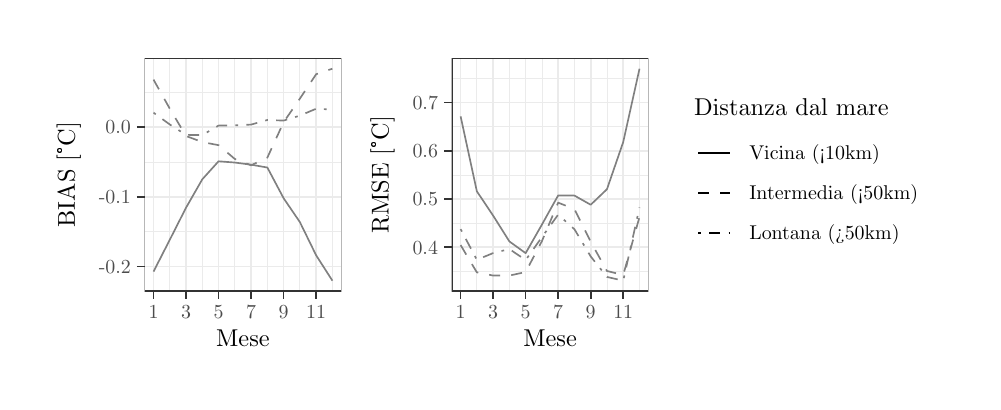
\begin{tikzpicture}[x=1pt,y=1pt]
\definecolor{fillColor}{RGB}{255,255,255}
\path[use as bounding box,fill=fillColor] (0,0) rectangle (341.43,128.04);
\begin{scope}
\path[clip] (  0.00,  0.00) rectangle (341.43,128.04);
\definecolor{drawColor}{RGB}{255,255,255}

\path[draw=drawColor,line width= 0.6pt,line join=round,line cap=round,fill=fillColor] (  0.00,  0.00) rectangle (341.43,128.04);
\end{scope}
\begin{scope}
\path[clip] (  5.50,  5.50) rectangle (118.85,122.54);
\definecolor{drawColor}{RGB}{255,255,255}
\definecolor{fillColor}{RGB}{255,255,255}

\path[draw=drawColor,line width= 0.6pt,line join=round,line cap=round,fill=fillColor] (  5.50,  5.50) rectangle (118.85,122.54);
\end{scope}
\begin{scope}
\path[clip] (118.85,  5.50) rectangle (335.93,122.54);
\definecolor{drawColor}{RGB}{255,255,255}
\definecolor{fillColor}{RGB}{255,255,255}

\path[draw=drawColor,line width= 0.6pt,line join=round,line cap=round,fill=fillColor] (118.85,  5.50) rectangle (335.93,122.54);
\end{scope}
\begin{scope}
\path[clip] ( 42.24, 32.79) rectangle (113.35,117.04);
\definecolor{fillColor}{RGB}{255,255,255}

\path[fill=fillColor] ( 42.24, 32.79) rectangle (113.35,117.04);
\definecolor{drawColor}{gray}{0.92}

\path[draw=drawColor,line width= 0.3pt,line join=round] ( 42.24, 54.36) --
	(113.35, 54.36);

\path[draw=drawColor,line width= 0.3pt,line join=round] ( 42.24, 79.52) --
	(113.35, 79.52);

\path[draw=drawColor,line width= 0.3pt,line join=round] ( 42.24,104.68) --
	(113.35,104.68);

\path[draw=drawColor,line width= 0.3pt,line join=round] ( 51.35, 32.79) --
	( 51.35,117.04);

\path[draw=drawColor,line width= 0.3pt,line join=round] ( 63.10, 32.79) --
	( 63.10,117.04);

\path[draw=drawColor,line width= 0.3pt,line join=round] ( 74.86, 32.79) --
	( 74.86,117.04);

\path[draw=drawColor,line width= 0.3pt,line join=round] ( 86.61, 32.79) --
	( 86.61,117.04);

\path[draw=drawColor,line width= 0.3pt,line join=round] ( 98.36, 32.79) --
	( 98.36,117.04);

\path[draw=drawColor,line width= 0.3pt,line join=round] (110.11, 32.79) --
	(110.11,117.04);

\path[draw=drawColor,line width= 0.6pt,line join=round] ( 42.24, 41.77) --
	(113.35, 41.77);

\path[draw=drawColor,line width= 0.6pt,line join=round] ( 42.24, 66.94) --
	(113.35, 66.94);

\path[draw=drawColor,line width= 0.6pt,line join=round] ( 42.24, 92.10) --
	(113.35, 92.10);

\path[draw=drawColor,line width= 0.6pt,line join=round] ( 45.47, 32.79) --
	( 45.47,117.04);

\path[draw=drawColor,line width= 0.6pt,line join=round] ( 57.23, 32.79) --
	( 57.23,117.04);

\path[draw=drawColor,line width= 0.6pt,line join=round] ( 68.98, 32.79) --
	( 68.98,117.04);

\path[draw=drawColor,line width= 0.6pt,line join=round] ( 80.73, 32.79) --
	( 80.73,117.04);

\path[draw=drawColor,line width= 0.6pt,line join=round] ( 92.48, 32.79) --
	( 92.48,117.04);

\path[draw=drawColor,line width= 0.6pt,line join=round] (104.24, 32.79) --
	(104.24,117.04);
\definecolor{drawColor}{gray}{0.50}

\path[draw=drawColor,line width= 0.6pt,line join=round] ( 45.47, 39.89) --
	( 51.35, 51.40) --
	( 57.23, 63.00) --
	( 63.10, 73.25) --
	( 68.98, 79.76) --
	( 74.86, 79.30) --
	( 80.73, 78.53) --
	( 86.61, 77.50) --
	( 92.48, 66.41) --
	( 98.36, 57.79) --
	(104.24, 45.78) --
	(110.11, 36.62);

\path[draw=drawColor,line width= 0.6pt,dash pattern=on 4pt off 4pt ,line join=round] ( 45.47,109.27) --
	( 51.35, 98.77) --
	( 57.23, 88.89) --
	( 63.10, 86.70) --
	( 68.98, 85.58) --
	( 74.86, 80.59) --
	( 80.73, 78.31) --
	( 86.61, 81.09) --
	( 92.48, 93.89) --
	( 98.36,102.39) --
	(104.24,111.24) --
	(110.11,113.21);

\path[draw=drawColor,line width= 0.6pt,dash pattern=on 1pt off 3pt on 4pt off 3pt ,line join=round] ( 45.47, 97.33) --
	( 51.35, 93.06) --
	( 57.23, 89.30) --
	( 63.10, 89.23) --
	( 68.98, 92.66) --
	( 74.86, 92.75) --
	( 80.73, 93.02) --
	( 86.61, 94.68) --
	( 92.48, 94.47) --
	( 98.36, 96.26) --
	(104.24, 98.75) --
	(110.11, 98.45);
\definecolor{drawColor}{gray}{0.20}

\path[draw=drawColor,line width= 0.6pt,line join=round,line cap=round] ( 42.24, 32.79) rectangle (113.35,117.04);
\end{scope}
\begin{scope}
\path[clip] (  0.00,  0.00) rectangle (341.43,128.04);
\definecolor{drawColor}{gray}{0.30}

\node[text=drawColor,anchor=base east,inner sep=0pt, outer sep=0pt, scale=  0.72] at ( 37.29, 39.31) {-0.2};

\node[text=drawColor,anchor=base east,inner sep=0pt, outer sep=0pt, scale=  0.72] at ( 37.29, 64.47) {-0.1};

\node[text=drawColor,anchor=base east,inner sep=0pt, outer sep=0pt, scale=  0.72] at ( 37.29, 89.64) {0.0};
\end{scope}
\begin{scope}
\path[clip] (  0.00,  0.00) rectangle (341.43,128.04);
\definecolor{drawColor}{gray}{0.20}

\path[draw=drawColor,line width= 0.6pt,line join=round] ( 39.49, 41.77) --
	( 42.24, 41.77);

\path[draw=drawColor,line width= 0.6pt,line join=round] ( 39.49, 66.94) --
	( 42.24, 66.94);

\path[draw=drawColor,line width= 0.6pt,line join=round] ( 39.49, 92.10) --
	( 42.24, 92.10);
\end{scope}
\begin{scope}
\path[clip] (  0.00,  0.00) rectangle (341.43,128.04);
\definecolor{drawColor}{gray}{0.20}

\path[draw=drawColor,line width= 0.6pt,line join=round] ( 45.47, 30.04) --
	( 45.47, 32.79);

\path[draw=drawColor,line width= 0.6pt,line join=round] ( 57.23, 30.04) --
	( 57.23, 32.79);

\path[draw=drawColor,line width= 0.6pt,line join=round] ( 68.98, 30.04) --
	( 68.98, 32.79);

\path[draw=drawColor,line width= 0.6pt,line join=round] ( 80.73, 30.04) --
	( 80.73, 32.79);

\path[draw=drawColor,line width= 0.6pt,line join=round] ( 92.48, 30.04) --
	( 92.48, 32.79);

\path[draw=drawColor,line width= 0.6pt,line join=round] (104.24, 30.04) --
	(104.24, 32.79);
\end{scope}
\begin{scope}
\path[clip] (  0.00,  0.00) rectangle (341.43,128.04);
\definecolor{drawColor}{gray}{0.30}

\node[text=drawColor,anchor=base,inner sep=0pt, outer sep=0pt, scale=  0.72] at ( 45.47, 22.91) {1};

\node[text=drawColor,anchor=base,inner sep=0pt, outer sep=0pt, scale=  0.72] at ( 57.23, 22.91) {3};

\node[text=drawColor,anchor=base,inner sep=0pt, outer sep=0pt, scale=  0.72] at ( 68.98, 22.91) {5};

\node[text=drawColor,anchor=base,inner sep=0pt, outer sep=0pt, scale=  0.72] at ( 80.73, 22.91) {7};

\node[text=drawColor,anchor=base,inner sep=0pt, outer sep=0pt, scale=  0.72] at ( 92.48, 22.91) {9};

\node[text=drawColor,anchor=base,inner sep=0pt, outer sep=0pt, scale=  0.72] at (104.24, 22.91) {11};
\end{scope}
\begin{scope}
\path[clip] (  0.00,  0.00) rectangle (341.43,128.04);
\definecolor{drawColor}{RGB}{0,0,0}

\node[text=drawColor,anchor=base,inner sep=0pt, outer sep=0pt, scale=  0.88] at ( 77.79, 12.71) {Mese};
\end{scope}
\begin{scope}
\path[clip] (  0.00,  0.00) rectangle (341.43,128.04);
\definecolor{drawColor}{RGB}{0,0,0}

\node[text=drawColor,rotate= 90.00,anchor=base,inner sep=0pt, outer sep=0pt, scale=  0.88] at ( 17.06, 74.91) {BIAS [\textdegree C]};
\end{scope}
\begin{scope}
\path[clip] (153.21, 32.79) rectangle (224.31,117.04);
\definecolor{fillColor}{RGB}{255,255,255}

\path[fill=fillColor] (153.21, 32.79) rectangle (224.31,117.04);
\definecolor{drawColor}{gray}{0.92}

\path[draw=drawColor,line width= 0.3pt,line join=round] (153.21, 39.95) --
	(224.31, 39.95);

\path[draw=drawColor,line width= 0.3pt,line join=round] (153.21, 57.39) --
	(224.31, 57.39);

\path[draw=drawColor,line width= 0.3pt,line join=round] (153.21, 74.83) --
	(224.31, 74.83);

\path[draw=drawColor,line width= 0.3pt,line join=round] (153.21, 92.27) --
	(224.31, 92.27);

\path[draw=drawColor,line width= 0.3pt,line join=round] (153.21,109.71) --
	(224.31,109.71);

\path[draw=drawColor,line width= 0.3pt,line join=round] (162.31, 32.79) --
	(162.31,117.04);

\path[draw=drawColor,line width= 0.3pt,line join=round] (174.07, 32.79) --
	(174.07,117.04);

\path[draw=drawColor,line width= 0.3pt,line join=round] (185.82, 32.79) --
	(185.82,117.04);

\path[draw=drawColor,line width= 0.3pt,line join=round] (197.57, 32.79) --
	(197.57,117.04);

\path[draw=drawColor,line width= 0.3pt,line join=round] (209.32, 32.79) --
	(209.32,117.04);

\path[draw=drawColor,line width= 0.3pt,line join=round] (221.08, 32.79) --
	(221.08,117.04);

\path[draw=drawColor,line width= 0.6pt,line join=round] (153.21, 48.67) --
	(224.31, 48.67);

\path[draw=drawColor,line width= 0.6pt,line join=round] (153.21, 66.11) --
	(224.31, 66.11);

\path[draw=drawColor,line width= 0.6pt,line join=round] (153.21, 83.55) --
	(224.31, 83.55);

\path[draw=drawColor,line width= 0.6pt,line join=round] (153.21,100.99) --
	(224.31,100.99);

\path[draw=drawColor,line width= 0.6pt,line join=round] (156.44, 32.79) --
	(156.44,117.04);

\path[draw=drawColor,line width= 0.6pt,line join=round] (168.19, 32.79) --
	(168.19,117.04);

\path[draw=drawColor,line width= 0.6pt,line join=round] (179.94, 32.79) --
	(179.94,117.04);

\path[draw=drawColor,line width= 0.6pt,line join=round] (191.69, 32.79) --
	(191.69,117.04);

\path[draw=drawColor,line width= 0.6pt,line join=round] (203.45, 32.79) --
	(203.45,117.04);

\path[draw=drawColor,line width= 0.6pt,line join=round] (215.20, 32.79) --
	(215.20,117.04);
\definecolor{drawColor}{gray}{0.50}

\path[draw=drawColor,line width= 0.6pt,line join=round] (156.44, 96.00) --
	(162.31, 68.91) --
	(168.19, 60.13) --
	(174.07, 50.79) --
	(179.94, 46.56) --
	(185.82, 56.88) --
	(191.69, 67.42) --
	(197.57, 67.37) --
	(203.45, 64.05) --
	(209.32, 69.66) --
	(215.20, 86.72) --
	(221.08,113.21);

\path[draw=drawColor,line width= 0.6pt,dash pattern=on 4pt off 4pt ,line join=round] (156.44, 49.47) --
	(162.31, 39.62) --
	(168.19, 38.47) --
	(174.07, 38.46) --
	(179.94, 39.74) --
	(185.82, 50.91) --
	(191.69, 64.81) --
	(197.57, 62.49) --
	(203.45, 50.67) --
	(209.32, 40.13) --
	(215.20, 38.66) --
	(221.08, 59.64);

\path[draw=drawColor,line width= 0.6pt,dash pattern=on 1pt off 3pt on 4pt off 3pt ,line join=round] (156.44, 55.24) --
	(162.31, 44.16) --
	(168.19, 46.59) --
	(174.07, 48.04) --
	(179.94, 44.07) --
	(185.82, 52.35) --
	(191.69, 60.48) --
	(197.57, 55.20) --
	(203.45, 45.37) --
	(209.32, 37.97) --
	(215.20, 36.62) --
	(221.08, 63.04);
\definecolor{drawColor}{gray}{0.20}

\path[draw=drawColor,line width= 0.6pt,line join=round,line cap=round] (153.21, 32.79) rectangle (224.31,117.04);
\end{scope}
\begin{scope}
\path[clip] (  0.00,  0.00) rectangle (341.43,128.04);
\definecolor{drawColor}{gray}{0.30}

\node[text=drawColor,anchor=base east,inner sep=0pt, outer sep=0pt, scale=  0.72] at (148.26, 46.20) {0.4};

\node[text=drawColor,anchor=base east,inner sep=0pt, outer sep=0pt, scale=  0.72] at (148.26, 63.64) {0.5};

\node[text=drawColor,anchor=base east,inner sep=0pt, outer sep=0pt, scale=  0.72] at (148.26, 81.08) {0.6};

\node[text=drawColor,anchor=base east,inner sep=0pt, outer sep=0pt, scale=  0.72] at (148.26, 98.53) {0.7};
\end{scope}
\begin{scope}
\path[clip] (  0.00,  0.00) rectangle (341.43,128.04);
\definecolor{drawColor}{gray}{0.20}

\path[draw=drawColor,line width= 0.6pt,line join=round] (150.46, 48.67) --
	(153.21, 48.67);

\path[draw=drawColor,line width= 0.6pt,line join=round] (150.46, 66.11) --
	(153.21, 66.11);

\path[draw=drawColor,line width= 0.6pt,line join=round] (150.46, 83.55) --
	(153.21, 83.55);

\path[draw=drawColor,line width= 0.6pt,line join=round] (150.46,100.99) --
	(153.21,100.99);
\end{scope}
\begin{scope}
\path[clip] (  0.00,  0.00) rectangle (341.43,128.04);
\definecolor{drawColor}{gray}{0.20}

\path[draw=drawColor,line width= 0.6pt,line join=round] (156.44, 30.04) --
	(156.44, 32.79);

\path[draw=drawColor,line width= 0.6pt,line join=round] (168.19, 30.04) --
	(168.19, 32.79);

\path[draw=drawColor,line width= 0.6pt,line join=round] (179.94, 30.04) --
	(179.94, 32.79);

\path[draw=drawColor,line width= 0.6pt,line join=round] (191.69, 30.04) --
	(191.69, 32.79);

\path[draw=drawColor,line width= 0.6pt,line join=round] (203.45, 30.04) --
	(203.45, 32.79);

\path[draw=drawColor,line width= 0.6pt,line join=round] (215.20, 30.04) --
	(215.20, 32.79);
\end{scope}
\begin{scope}
\path[clip] (  0.00,  0.00) rectangle (341.43,128.04);
\definecolor{drawColor}{gray}{0.30}

\node[text=drawColor,anchor=base,inner sep=0pt, outer sep=0pt, scale=  0.72] at (156.44, 22.91) {1};

\node[text=drawColor,anchor=base,inner sep=0pt, outer sep=0pt, scale=  0.72] at (168.19, 22.91) {3};

\node[text=drawColor,anchor=base,inner sep=0pt, outer sep=0pt, scale=  0.72] at (179.94, 22.91) {5};

\node[text=drawColor,anchor=base,inner sep=0pt, outer sep=0pt, scale=  0.72] at (191.69, 22.91) {7};

\node[text=drawColor,anchor=base,inner sep=0pt, outer sep=0pt, scale=  0.72] at (203.45, 22.91) {9};

\node[text=drawColor,anchor=base,inner sep=0pt, outer sep=0pt, scale=  0.72] at (215.20, 22.91) {11};
\end{scope}
\begin{scope}
\path[clip] (  0.00,  0.00) rectangle (341.43,128.04);
\definecolor{drawColor}{RGB}{0,0,0}

\node[text=drawColor,anchor=base,inner sep=0pt, outer sep=0pt, scale=  0.88] at (188.76, 12.71) {Mese};
\end{scope}
\begin{scope}
\path[clip] (  0.00,  0.00) rectangle (341.43,128.04);
\definecolor{drawColor}{RGB}{0,0,0}

\node[text=drawColor,rotate= 90.00,anchor=base,inner sep=0pt, outer sep=0pt, scale=  0.88] at (130.41, 74.91) {RMSE [\textdegree C]};
\end{scope}
\begin{scope}
\path[clip] (  0.00,  0.00) rectangle (341.43,128.04);
\definecolor{fillColor}{RGB}{255,255,255}

\path[fill=fillColor] (235.31, 41.10) rectangle (330.43,108.73);
\end{scope}
\begin{scope}
\path[clip] (  0.00,  0.00) rectangle (341.43,128.04);
\definecolor{drawColor}{RGB}{0,0,0}

\node[text=drawColor,anchor=base west,inner sep=0pt, outer sep=0pt, scale=  0.88] at (240.81, 96.31) {Distanza dal mare};
\end{scope}
\begin{scope}
\path[clip] (  0.00,  0.00) rectangle (341.43,128.04);
\definecolor{fillColor}{RGB}{255,255,255}

\path[fill=fillColor] (240.81, 75.50) rectangle (255.26, 89.96);
\end{scope}
\begin{scope}
\path[clip] (  0.00,  0.00) rectangle (341.43,128.04);
\definecolor{drawColor}{RGB}{0,0,0}

\path[draw=drawColor,line width= 0.6pt,line join=round] (242.25, 82.73) -- (253.82, 82.73);
\end{scope}
\begin{scope}
\path[clip] (  0.00,  0.00) rectangle (341.43,128.04);
\definecolor{fillColor}{RGB}{255,255,255}

\path[fill=fillColor] (240.81, 61.05) rectangle (255.26, 75.50);
\end{scope}
\begin{scope}
\path[clip] (  0.00,  0.00) rectangle (341.43,128.04);
\definecolor{drawColor}{RGB}{0,0,0}

\path[draw=drawColor,line width= 0.6pt,dash pattern=on 4pt off 4pt ,line join=round] (242.25, 68.28) -- (253.82, 68.28);
\end{scope}
\begin{scope}
\path[clip] (  0.00,  0.00) rectangle (341.43,128.04);
\definecolor{fillColor}{RGB}{255,255,255}

\path[fill=fillColor] (240.81, 46.60) rectangle (255.26, 61.05);
\end{scope}
\begin{scope}
\path[clip] (  0.00,  0.00) rectangle (341.43,128.04);
\definecolor{drawColor}{RGB}{0,0,0}

\path[draw=drawColor,line width= 0.6pt,dash pattern=on 1pt off 3pt on 4pt off 3pt ,line join=round] (242.25, 53.82) -- (253.82, 53.82);
\end{scope}
\begin{scope}
\path[clip] (  0.00,  0.00) rectangle (341.43,128.04);
\definecolor{drawColor}{RGB}{0,0,0}

\node[text=drawColor,anchor=base west,inner sep=0pt, outer sep=0pt, scale=  0.72] at (260.76, 80.27) {Vicina (<10km)};
\end{scope}
\begin{scope}
\path[clip] (  0.00,  0.00) rectangle (341.43,128.04);
\definecolor{drawColor}{RGB}{0,0,0}

\node[text=drawColor,anchor=base west,inner sep=0pt, outer sep=0pt, scale=  0.72] at (260.76, 65.81) {Intermedia (<50km)};
\end{scope}
\begin{scope}
\path[clip] (  0.00,  0.00) rectangle (341.43,128.04);
\definecolor{drawColor}{RGB}{0,0,0}

\node[text=drawColor,anchor=base west,inner sep=0pt, outer sep=0pt, scale=  0.72] at (260.76, 51.36) {Lontana (>50km)};
\end{scope}
\end{tikzpicture}

  \caption{BIAS e RMSE delle stazioni italiane in funzione della distanza dal mare (quota < \qty{500}{\meter}).}\label{fig:sea-bias}
\end{figure}
